% ==============================================================================
% PHỤ LỤC (APPENDIX)
% ==============================================================================

\chapter*{PHỤ LỤC}
\addcontentsline{toc}{chapter}{Phụ lục}
\renewcommand{\thesection}{\Alph{section}}
\renewcommand{\theHsection}{appendix.\Alph{section}}
\setcounter{section}{0}
\counterwithin{figure}{section}
\renewcommand{\theHfigure}{appendix.\thesection.\arabic{figure}}
\counterwithout{lstlisting}{chapter}
\counterwithin{lstlisting}{section}

\section{Đối Chiếu Nguồn Gốc Báo Cáo và Mã Nguồn Thực Tế (Traceability Overview)}

Nhằm bảo đảm tính minh bạch học thuật, bản cập nhật phân biệt implementation hiện tại, artifact local lịch sử và benchmark được tài liệu hóa; các nguồn tương ứng được liệt kê dưới đây:

\begin{itemize}[leftmargin=1.5cm]
  \item \textbf{Chương 1 (Hiểu bài toán \& KPI)}: \path{docs/OVERVIEW.md}, \path{SETUP.md}.
  \item \textbf{Chương 2 (Khám phá EDA \& Thống kê)}: \path{data/gold/mining/eda_summary.json}, \path{src/mining/eda_engine.py}.
  \item \textbf{Chương 3 (Thu thập 3 tầng \& Lakehouse)}: \path{src/ingestion/arxiv_batch_harvester.py}, \path{src/storage/duckdb_engine.py}, \path{src/transformation/html_parser.py}, \path{src/indexing/qdrant_manager.py}.
  \item \textbf{Chương 4 (4 Trụ cột Khai phá Dữ liệu \& RAG)}: \path{src/mining/association_rules.py}, \path{src/mining/cluster_analysis.py}, \path{src/mining/graph_mining.py}, \path{src/mining/trend_anomaly_mining.py}, \path{backend/app/services/retrieval_service.py}.
  \item \textbf{Chương 5 (Đánh giá DeepEval \& Hiệu năng GPU)}: \path{docs/benchmarks/RAG_EVALUATION_REPORT_21_SAMPLES.md}, \path{docs/benchmarks/PERFORMANCE_BENCHMARK_REPORT.md}.
  \item \textbf{Chương 6 (Triển khai Vận hành)}: \path{README.md}, \path{.env_example}, \path{dags/}, \path{backend/app/main.py}.
\end{itemize}

\subsection{Mốc Đối Chiếu và Tính Tái Lập}
Quy ước của báo cáo: source xác nhận đường xử lý đã triển khai; artifact ghi đầu ra của một snapshot; benchmark ghi kết quả của một phép đo; ảnh giao diện minh họa cách hiển thị. Chứng cứ thuộc loại này không tự thay thế loại khác. Các phép tính bổ sung như số giao dịch hỗ trợ, tổng thời gian hoặc tỷ số đều được suy từ số đã lưu và ghi rõ giới hạn làm tròn; không có lần chạy mining/benchmark mới.

Mã nguồn: commit \texttt{f421707}, ngày 09/11/2026; ngày cập nhật báo cáo 25/11/2026. Không chạy lại mining hoặc benchmark; frontend/backend không bị sửa đổi. Các file JSON local được xem là snapshot lịch sử; manifest tham chiếu ngày 04/10/2026 không xác nhận mọi artifact đã được tái lập cùng một lần chạy.

DeepEval: report 05/10/2026 ghi commit \texttt{6cb1c52}, LanceDB, hơn 143 nghìn chunk. Hiệu năng phần cứng: report 19/10/2026. Các benchmark bổ sung giai đoạn 06--08/11/2026 nằm tại \path{logs/benchmarks/} (\path{chunking_ab/summary.json}, \path{rag_eval/report_retrieval.json}) và \path{notebooks/} (\path{laya_onnx_20261108-2053_seed0/RUN_INFO.json}, \path{laya_finetune/report_seed0.json}). Các số quy mô citation và landmark chưa có artifact đối chiếu được loại khỏi bảng kết quả.

\subsection{Nguồn Bổ Sung cho Kiến Trúc Mới}
\begin{itemize}
\item \path{src/storage/chunk_store.py}, \path{src/indexing/qdrant_manager.py}: schema chunk, payload tối thiểu, hydrate và compaction.
\item \path{src/ingestion/queue_consumer.py}, \path{dags/dag_tier1_realtime_stream.py}, \path{dags/dag_tier2_near_past_harvest.py}, \path{dags/dag_compact_silver.py}: hai stage, lịch và backpressure.
\item \path{src/utils/hasher.py}, \path{src/storage/known_papers.py}, \path{src/transformation/silver_writer.py}: abstract hash và dedup.
\item \path{backend/app/core/config.py}, \path{backend/app/schemas/chat.py}, \path{backend/app/services/rag_service.py}: mặc định reranker/chat.
\item \path{benchmarks/rag_eval/}, \path{benchmarks/laya_finetune/}, \path{benchmarks/chunking_ab/}: bộ đánh giá Retrieval v1, fine-tune Laya ONNX và Chunking A/B.
\end{itemize}

\subsection{Bộ Ảnh Chụp Tự Động Ngày 23/11/2026}
Bộ ảnh gồm Pipeline, metadata Bronze, EDA Silver, hai ma trận tương quan, GMM và manifest Gold. PNG gốc, nguồn API, thời điểm chụp và SHA-256 nằm trong \path{figures/captured_20261123_082337/manifest.json}; các response dùng đối chiếu nằm trong thư mục \path{evidence/} cùng bộ ảnh.

Hình~\ref{fig:gold_manifest_capture} hiển thị cấu trúc tệp manifest định danh các sản phẩm khai phá dữ liệu thuộc tầng Gold, lưu trữ các siêu dữ liệu cấu hình và đường dẫn artifact phục vụ việc truy xuất và tái lập kết quả.
\begin{figure}[!htbp]
\centering
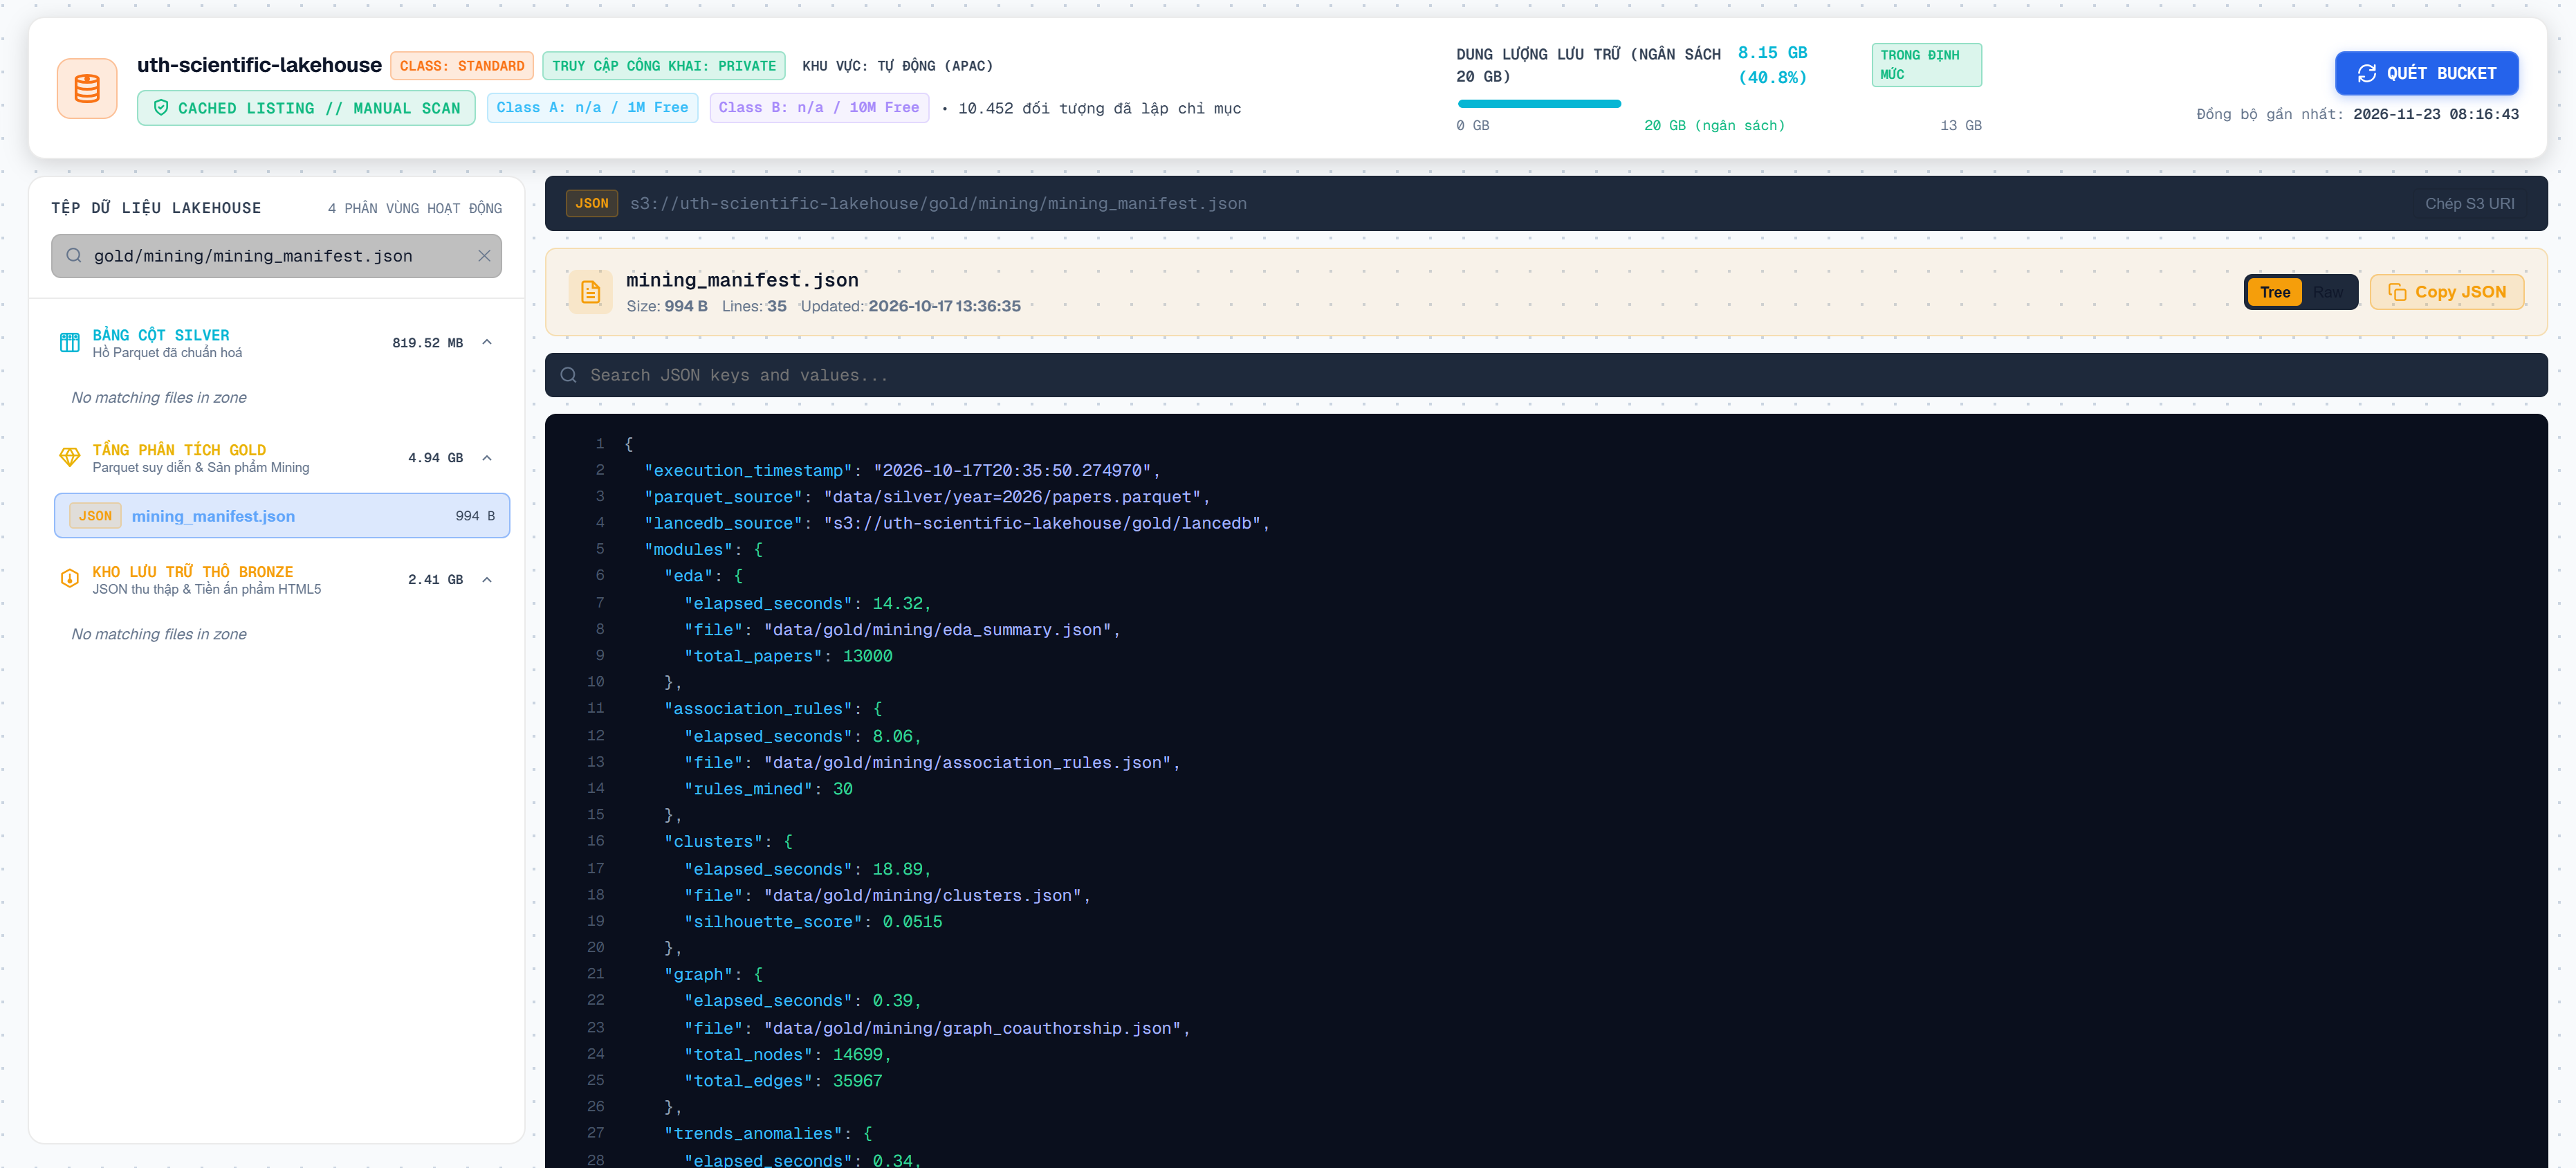
\includegraphics[width=\linewidth,height=0.68\textheight,keepaspectratio]{figures/captured_20261123_082337/07_gold_mining_manifest.png}
\caption[Manifest của các sản phẩm khai phá Gold]{Manifest của các sản phẩm khai phá Gold}
\label{fig:gold_manifest_capture}
\ReportNote{Nguồn: Tệp kê khai định danh và thông số các sản phẩm khai phá dữ liệu tầng Gold (\path{gold/mining/mining_manifest.json}).}
\end{figure}
\FloatBarrier

\section{Trích Đoạn Mã Nguồn Tiêu Biểu (Key Code Listings)}

\subsection{Thuật toán Khai phá Luật Kết hợp FP-Growth với Khử Trùng lặp Đối xứng}
Đoạn mã trích từ \path{src/mining/association_rules.py} thể hiện quá trình một-nóng hóa giao dịch, dựng cây FP-Tree và lọc luật đối xứng theo giá trị Lift và Confidence:

\begin{lstlisting}[language=Python, caption={Khử trùng lặp luật đối xứng trong AssociationRuleMiner}]
# Trich doan tu src/mining/association_rules.py
te = TransactionEncoder()
te_ary = te.fit_transform(transactions)
df_encoded = pd.DataFrame(te_ary, columns=te.columns_)

# Khai pha tap muc pho bien bang FP-Growth
frequent_itemsets = fpgrowth(df_encoded, min_support=min_support, use_colnames=True)

# Sinh luat ket hop theo do nang Lift
rules = association_rules(frequent_itemsets, metric="lift", min_threshold=min_lift)
rules = rules.assign(_lift_key=rules["lift"].round(6))
sorted_rules = rules.sort_values(by=["_lift_key", "confidence"], ascending=[False, False])

# Khu trung lap luat doi xung: giu lai chieu co Confidence cao hon
deduped_rows = []
seen_pairs = set()
for _, row in sorted_rules.iterrows():
    ant = tuple(sorted(list(row["antecedents"])))
    con = tuple(sorted(list(row["consequents"])))
    pair_key = frozenset([ant, con])
    if pair_key in seen_pairs:
        continue
    seen_pairs.add(pair_key)
    deduped_rows.append(row)
\end{lstlisting}

\subsection{Cơ chế Tăng cường Điểm Uy tín PageRank trong Thuật toán Tìm kiếm Lai (RAG Retrieval)}
Đoạn mã trích từ \path{backend/app/services/retrieval_service.py} thể hiện việc ánh xạ tác giả bài báo với các nút có điểm PageRank cao trong artifact graph được nạp (citation hoặc đồng tác giả):

\begin{lstlisting}[language=Python, caption={Bộ nhân uy tín PageRank Authority Multiplier}]
# Trich doan tu backend/app/services/retrieval_service.py
def _match_authority(self, authors: List[str]) -> Tuple[float, Optional[str]]:
    """Anh xa tac gia cua doan trich voi cac nut co PageRank cao trong mang luoi."""
    self._ensure_graph_and_rules()
    if not authors or not self.influencers:
        return 0.0, None

    best_pr = 0.0
    best_author = None
    for a in authors:
        a_lower = a.lower().strip()
        for inf in self.influencers:
            if inf["author_clean"] in a_lower or a_lower in inf["author_clean"]:
                if inf["pagerank"] > best_pr:
                    best_pr = inf["pagerank"]
                    best_author = a

    if best_pr > 0.0:
        norm_pr = min(1.0, best_pr / max(1e-6, self.max_pagerank))
        return norm_pr, best_author
    return 0.0, None
\end{lstlisting}

\Needspace{9\baselineskip}
\subsection{Phát hiện Bài báo Dị biệt Cấu trúc Bằng Rừng Cô Lập với Chuẩn hóa $\log(1+x)$}
Đoạn mã trích từ \path{src/mining/trend_anomaly_mining.py}:

\begin{lstlisting}[language=Python, caption={Isolation Forest tren dac trung log1p}]
# Trich doan tu src/mining/trend_anomaly_mining.py
feature_cols = [
    "total_math_count",
    "total_words",
    "total_sections",
    "author_count",
    "category_count",
]
X_raw = df[feature_cols].fillna(0).values.astype(np.float64)
# Chuan hoa log(1+x) de giam do lech phan phoi duoi dai
X_log = np.log1p(X_raw)

iso_forest = IsolationForest(
    contamination=contamination,
    random_state=42,
    n_estimators=100,
)
preds = iso_forest.fit_predict(X_log)
anomaly_scores = iso_forest.score_samples(X_log)
df["is_anomaly"] = preds == -1
\end{lstlisting}


\subsection{Payload Vector Tối Thiểu và Hydrate từ Silver}
Đoạn mã được trích từ \path{src/storage/chunk_store.py} và \path{src/indexing/qdrant_manager.py}, đối chiếu tới commit \texttt{f421707}. Qdrant giữ trường định danh/lọc; kết quả thiếu text được bổ sung từ bảng chunk Silver. Các dấu ngắt dưới đây phân tách các đoạn trích từ hai module, không biểu diễn một script độc lập.
\lstinputlisting[language=Python,caption={Trường payload và hydrate nội dung từ Silver},label={lst:payload_hydrate}]{listings/qdrant_payload_hydrate.py}

\subsection{Ghi Silver Chunks Trước Khi Upsert Vector}
Đoạn trích từ \path{src/ingestion/queue_consumer.py}, đối chiếu tới commit \texttt{f421707}, cho thấy thứ tự ghi chunk table và nhánh bỏ qua các bài thuộc phân vùng ghi thất bại. Chỉ các đoạn liên quan được giữ; vị trí lược bớt được đánh dấu bằng chú thích.
\lstinputlisting[language=Python,caption={Thứ tự ghi Silver chunks và upsert Qdrant},label={lst:silver_before_vector}]{listings/silver_before_vector.py}

\Needspace{12\baselineskip}
\section{Hướng Dẫn Cài Đặt và Khởi Chạy Nhanh Dự Án}

\subsection{Cài đặt môi trường Python}
\begin{lstlisting}[language=bash]
# 1. Tao moi truong ao
python -m venv .venv

# 2. Kich hoat moi truong ao (Windows PowerShell)
.\.venv\Scripts\Activate.ps1

# 3. Cai dat cac goi thu vien phu thuoc
pip install --upgrade pip
pip install -r requirements.txt
pip install -e .
\end{lstlisting}

\subsection{Các lệnh kiểm thử tham khảo}
\begin{lstlisting}[language=bash]
# Unit tests; integration tests require configured external services
pytest tests/unit/ -v
pytest tests/integration/ -v
\end{lstlisting}
